\documentclass[12pt]{article}
\usepackage[hungarian]{babel}
\selectlanguage{hungarian}
\usepackage[utf8]{inputenc}
\usepackage[T1]{fontenc}
\usepackage{graphicx,latexsym,amsmath}
\usepackage{blkarray}
\usepackage{wrapfig}
\usepackage{tikz}
\usepackage[makeroom]{cancel}
\usetikzlibrary{arrows,automata}

\pdfpageheight\paperheight
\pdfpagewidth\paperwidth
\setlength\topmargin{-7mm} \setlength\oddsidemargin{-0cm}
\setlength\textheight{22cm} \setlength\textwidth{15.8cm}
\setlength\columnsep{0.25in}  \newlength\titlebox \setlength\titlebox{2.00in}
\setlength\headheight{5pt}   \setlength\headsep{0pt}
\setlength\footskip{1.9cm}
\setlength\leftmargin{0.0in}

\usepackage{makecell}
\newcolumntype{x}[1]{>{\centering\arraybackslash}p{#1}}
\newcommand\diag[4]{%
	\multicolumn{1}{p{#2}|}{\hskip-\tabcolsep
		$\vcenter{\begin{tikzpicture}[baseline=0,anchor=south west,inner sep=#1]
			\path[use as bounding box] (0,0) rectangle 
			(#2+2\tabcolsep,\baselineskip);
			\node[minimum width={#2+2\tabcolsep-\pgflinewidth},
			minimum  height=\baselineskip+\extrarowheight-\pgflinewidth] (box) 
			{};
			\draw[line cap=round] (box.north west) -- (box.south east);
			\node[anchor=south west] at (box.south west) {#3};
			\node[anchor=north east] at (box.north east) {#4};
			\end{tikzpicture}}$\hskip-\tabcolsep}}

\title{10. gyakorlat -- Mintaillesztés és moduláris hatványozás}
\date{}
\begin{document}
	
	\maketitle
	
	\noindent 1. Adjunk meg egy véges állapotú determinisztikus automatát, ami 
	a \texttt{P='aababa'} minta illesztését hajtja végre!
	
	\begin{table}[h!]
		\centering
		\begin{tabular}{cc}
			\\
			$\delta(q_0,a)=q_1$ & $\delta(q_0,b)=q_0$ \\
			$\delta(q_1,a)=q_2$ & $\delta(q_1,b)=q_0$ \\
			$\delta(q_2,a)=q_2$ & $\delta(q_2,b)=q_3$ \\
			$\delta(q_3,a)=q_4$ & $\delta(q_3,b)=q_0$ \\
			$\delta(q_4,a)=q_2$ & $\delta(q_4,b)=q_5$ \\
			$\delta(q_5,a)=q_6$ & $\delta(q_5,b)=q_0$ \\
			$\delta(q_6,a)=q_2$ & $\delta(q_6,b)=q_0$ \\
		\end{tabular} vagy kicsit olvashatóbban
		\begin{tabular}{c|cc}
			\diag{0em}{1em}{$Q$}{$\Sigma$} &  $a$  &  $b$ \\ \hline
			$q_0$ & $q_1$ & $q_0$ \\
			$q_1$ & $q_2$ & $q_0$ \\
			$q_2$ & $q_2$ & $q_3$ \\
			$q_3$ & $q_4$ & $q_0$ \\
			$q_4$ & $q_2$ & $q_5$ \\
			$q_5$ & $q_6$ & $q_0$ \\
			$q_6$ & $q_2$ & $q_0$ \\
		\end{tabular}
		\caption{\texttt{P} minta illesztését vizsgáló automata $\delta$ 
		állapotátmenet-függvénye.}
	\end{table}
	
	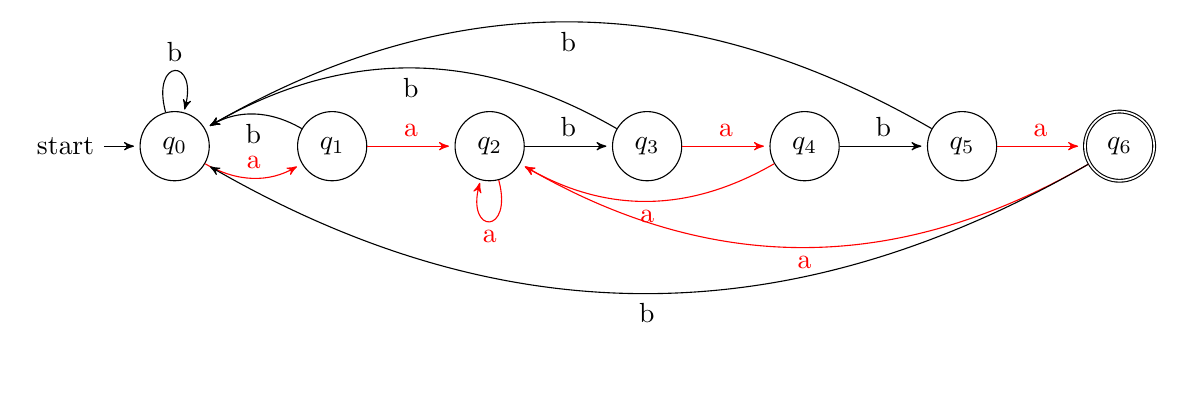
\begin{tikzpicture}[>=stealth',shorten >=2pt,auto,node distance=2cm]
	\node[initial,state]         (q0) {$q_0$};
	\node[state]         (q1) [right of=q0] {$q_1$};
	\node[state]         (q2) [right of=q1] {$q_2$};
	\node[state]         (q3) [right of=q2] {$q_3$};
	\node[state]         (q4) [right of=q3] {$q_4$};
	\node[state]         (q5) [right of=q4] {$q_5$};
	\node[state,accepting] (q6) [right of=q5] {$q_6$};
	
	\path[->]
	(q0) edge [bend right,color=red] node {a} (q1)
	edge [loop above] node {b} (q0)
	(q1) edge [color=red]node {a} (q2)
	edge [bend right] node {b} (q0)
	(q2) edge node {b} (q3)
	edge [loop below,color=red] node {a} (q2)
	(q3) edge [color=red] node {a} (q4)
	edge [bend right]  node {b} (q0)
	(q4) edge node {b} (q5)
	edge [bend left,color=red] node {a} (q2)
	(q5) edge [color=red] node {a} (q6)
	edge [bend right] node {b} (q0)
	(q6) edge [bend left,color=red] node {a} (q2)
	edge [bend left] node {b} (q0);
	\end{tikzpicture}
	
	Milyen állapotokat érint az automata a \texttt{T='aaabaababa'} input 
	feldolgozása során?
	\begin{table}[h!]
	    \centering
    	\begin{tabular}{c|ccccccccccc}
	    	i    &   0  & 1 & 2 & 3 & 4 & 5 & 6 & 7 & 8 & 9 & 10 \\ \hline
	    	T[i] &  --  & a & a & a & b & a & a & b & a & b &  a \\
	    	$q_i$&$q_0$ &$q_1$ &$q_2$ &$q_2$ &$q_3$ &$q_4$ &$q_2$ &$q_3$ &$q_4$ 
	    	&$q_5$ & \fbox{$q_6$}
	    \end{tabular}
	\end{table}
	
\noindent 2. Adjuk meg a Knuth-Morris-Pratt algoritmus által a \texttt{P} 
mintához meghatározott $\pi: \{1,2,\ldots, m\} \rightarrow \{0,1,\ldots, m-1\}$ 
prefixfüggvényt!
	
	\textbf{Előtte egy kis emlékeztető.}
	
	$\mathtt{P}_i$ jelölje \texttt{P}-nek az $i$ hosszúságú prefixét 
	(kezdőszeletét), azaz pl. $\mathtt{P}_3=aab$, $\mathtt{P}_2=aa$, 
	$\mathtt{P}_1=a$, illetve $\mathtt{P}_0=\epsilon$, ahol $\epsilon$ az üres 
	szót jelöli.
	
	$\mathtt{X} \sqsupset \mathtt{Y}$ jelölje azt, ha \texttt{X} sztring 
	szuffixe \texttt{Y}-nak (azaz teljesül, hogy \texttt{Y} végződése 
	megegyezik magával \texttt{X}-szel). 
	(Pl.~$\mathtt{\underline{aaba}}\sqsupset\mathtt{cac\underline{aaba}}$, 
	ugyanakkor 
	$\mathtt{\underline{aaba}}\not\sqsupset\mathtt{cac\underline{aab\textcolor{red}{\textbf{b}}}}$.)
	
	Megjegyzés: Az $\mathtt{Y} \sqsupset \mathtt{Y}$, valamint az $\epsilon 
	\sqsupset \mathtt{Y}$ relációk triviálisan teljesülnek minden 
	$\mathtt{Y}$-ra.
	
	Ezek után legyen $\pi[q]=\max\{k : k < q \wedge \mathtt{P}_k \sqsupset 
	\mathtt{P}_q\}$, azaz a $q$-hoz rendelt prefixfüggvény értéke legyen 
	\texttt{P} azon leghosszabb ($q$-nál rövidebb) prefixének hosszával 
	egyenlő, ami valódi (vele nem megegyező) szuffixe $\mathtt{P}_q$-nak.
	
	Pl.~$\pi[4]=1$, mivel
	\begin{itemize}
		\item 
		$\underline{aab}=\mathtt{P_3}\not\sqsupset\mathtt{P_4}=a\underline{aba}$
		\item 
		$\underline{aa}=\mathtt{P_2}\not\sqsupset\mathtt{P_4}=aa\underline{ba}$
		\item 
		$\underline{a}=\mathtt{P_1}\sqsupset\mathtt{P_4}=aab\underline{a}$.
	\end{itemize}
	
	\begin{tabular}{c|ccccccc}
		i       &   0  & 1 & 2 & 3 & 4 & 5 & 6 \\ \hline
		P[i]    &  --  & a & a & b & a & b & a \\
		$\pi[i]$&      & 0 & 1 & 0 & 1 & 0 & 1
	\end{tabular}

\noindent 3. Rabin-Karp algoritmussal döntsük el, hogy a 
$\texttt{T=3613203214}$ 
input kapcsán mely indexeiről kezdődhet a $\texttt{P=321}$ mintára való 
illeszkedés a $h(x) = x \mod 11$ hasítófüggvény használata mellett?

0. index: $361 \mod 11 = 9$

1. index: $613 \mod 11 = 10*(9 - 1 * 3) + 3 \mod 11 = 8$

2. index: $132 \mod 11 = 10*(8 - 1 * 6) + 2 \mod 11 = 0$

3. index: $320 \mod 11 = 10*(0 - 1 * 1) + 0 \mod 11 = 1$

4. index: $203 \mod 11 = 10*(1 - 1 * 3) + 3 \mod 11 = 5$

5. index: $032 \mod 11 = 10*(5 - 1 * 2) + 2 \mod 11 = 10$

6. index: $321 \mod 11 = 10*(10 - 1 * 0) + 1 \mod 11 = 2$

7. index: $214 \mod 11 = 10*(2 - 1 * 3) + 4 \mod 11 = 5$

Milyen karakternek kéne a \texttt{T} minta következő pozícióján álljon, hogy a 
Rabin-Karp algoritmus tévesen megvizsgálja az illeszkedést?

$14y \mod 11 = 10*(5-1*2)+y \mod 11 = 2$

\noindent 4. Moduláris hatványozás segítségével határozzuk meg a $d=7^{13} \mod 
17$ kifejezés értékét?

$13 = 1101b$

$d=1 \xrightarrow{1/a} d=(1*1) \mod 17 = 1 \xrightarrow{1/b} d=(1*7) \mod 17 = 
7 \xrightarrow{2/a} d=(7*7) \mod 17 = 15 \xrightarrow{2/b} d=(15*7) \mod 17 = 
3 \xrightarrow{3/a} d=(3*3) \mod 17 = 9 \xrightarrow{4/a} d=(9*9) \mod 17 
= 13 \xrightarrow{4/b} d=(13*7) \mod 17 = 91 \mod 17 = \boxed{6}$

\end{document}